% ==============================================================================
% CHAPTER 1: Introduction
% ==============================================================================

\chapter{Introduction}
\label{ch:introduction}

\lettrine[lines=3]{T}{he physical layout} of analog integrated circuits (ICs) remains a highly manual, time-consuming phase of the semiconductor design cycle. While digital physical design flows have achieved near-complete automation through logic synthesis and automated placement and routing (P\&R) algorithms, analog layout continues to rely on the manual expertise of physical design engineers. This discrepancy is primarily due to the complex nature of analog design, where layout geometries directly influence performance metrics such as offset voltage, noise margins, and parasitic mismatch.

Analog layout requires careful management of spatial symmetry, thermal gradients, latch-up clearances, and electrical shielding. Manual layout processes are slow and prone to errors, causing a bottleneck that delays time-to-market. Recent efforts in electronic design automation (EDA) have attempted to close this gap by applying machine learning (ML) and optimization techniques to automate analog physical design. However, these systems often face challenges, such as the high complexity of sub-micron process design rules and difficulty in adapting to designer feedback.

This thesis introduces a decoupled, multi-agent layout automation framework that separates high-level strategic reasoning from low-level geometric compaction. By leveraging Large Language Models (LLMs) organized as a cooperative state-machine (LangGraph) alongside deterministic physical layout compilers, the proposed framework automates the schematic-to-layout flow while maintaining design rule correctness and support for interactive designer edits.

% ==============================================================================
\section{Background and Context}
\label{sec:background}

Over the past four decades, the semiconductor industry has witnessed exponential growth in integration density and performance, primarily driven by digital design automation. In the digital domain, logical functions are synthesized from high-level hardware description languages (such as Verilog or VHDL) into standardized cell footprints (e.g., standard cells). These standard cells have fixed heights, uniform power rails, and predetermined electrical characteristics, enabling automated routers and placers to treat the physical layout as a discrete optimization problem.

In contrast, analog circuit design remains fundamentally non-standardized. Analog designs utilize custom device sizing (width, length, finger numbers, and multiplier values) tailored to specific gain, bandwidth, noise, and power specifications. Devices cannot be easily abstracted into uniform standard cells; instead, they are placed in a custom, continuous physical space. Furthermore, the physical proximity of devices in an analog layout induces electrical and physical coupling effects that do not exist in digital abstractions. For instance, the threshold voltage ($V_{th}$) and mobility ($\mu$) of a transistor are heavily dependent on its distance to well boundaries and neighboring active oxide areas. Because of this high sensitivity, the layout process is highly iterative, requiring multiple loops of schematic sizing, physical layout creation, parasitic extraction (PEX), and post-layout simulation. The layout phase alone typically accounts for more than $50\%$ of the total mixed-signal design time, creating a major productivity bottleneck.

% ==============================================================================
\section{Challenges in Analog Layout Automation}
\label{sec:motivation}

The primary obstacles preventing the full automation of analog physical design stem from the complex physical constraints of analog integrated circuits. These challenges can be grouped into five primary categories:

\subsection{Geometric and Symmetrical Matching}
Symmetrical matching is critical for minimizing the mismatch between matched transistor pairs, such as differential inputs, current mirror pairs, and active loads. Mismatch arises from random and systematic process variations during fabrication, including oxide thickness variations, channel doping fluctuations, and implant gradients. To mitigate these variations, analog layout designers employ specialized matching configurations:
\begin{itemize}
    \item \textbf{Interdigitation:} Splitting transistors into multiple fingers and interleaving them (e.g., $ABAB$ or $ABBA$) to average out linear gradients across the active channel.
    \item \textbf{Common-Centroid:} Arranging the fingers of two matched transistors symmetrically around a central point in a 2D matrix (e.g., $A B / B A$). This configuration cancels out first-order linear gradients in both the $x$ and $y$ directions:
    \begin{equation}
        V_{th}(x,y) = ax + by + c \implies \Delta V_{th} = V_{th,A} - V_{th,B} = 0
    \end{equation}
    where $a$ and $b$ represent the linear spatial gradient coefficients, and $c$ is the nominal threshold voltage.
    \item \textbf{Dummy Devices:} Placing inactive, dummy transistors at the outer edges of the active array to ensure that all active fingers experience identical etching, photolithography, and oxide growth boundaries.
\end{itemize}
Automated placers must recognize these matching pairs from netlist structures and enforce strict 1D or 2D symmetry constraints, matching coordinate centers while routing symmetric nets identically.

\subsection{Layout Dependent Effects (LDE)}
In deep sub-micron nodes (e.g., CMOS nodes at 28nm and below, FinFET, and nanosheet architectures), the electrical performance of a transistor is modulated by its physical placement relative to surrounding oxide and well boundaries. The two most prominent effects are:
\begin{enumerate}
    \item \textbf{Well Proximity Effect (WPE):} During high-energy ion implantation of the well (e.g., N-well in a P-substrate), ions scatter from the photoresist mask edge into the adjacent silicon. Transistors placed close to the well boundary experience a significant shift in well doping concentration, causing a shift in threshold voltage ($\Delta V_{th}$).
    \begin{thesiscallout}{Well Proximity Effect (WPE) Model}
    WPE threshold voltage shift is modeled as:
    \begin{equation}
        \Delta V_{th} \approx \frac{C_{\text{WPE}}}{(d_{\text{well}} + d_0)^{\beta}}
    \end{equation}
    where $d_{\text{well}}$ is the distance between the transistor gate and the N-well edge, and $C_{\text{WPE}}$, $d_0$, and $\beta$ are process-dependent fitting parameters.
    \end{thesiscallout}
    \item \textbf{Shallow Trench Isolation (STI) Stress:} Shallow trench isolation trenches are filled with silicon dioxide ($SiO_2$), which has a different thermal expansion coefficient than silicon. This difference induces mechanical stress on the adjacent active channels, shifting carrier mobility ($\mu$) and threshold voltage. The stress level depends heavily on the Length of active OD ($L_{OD}$), which is the distance between the gate and the STI boundary.
    \begin{thesiscallout}{STI Mechanical Stress Model}
    STI stress shifts the nominal drain current by:
    \begin{equation}
        \frac{\Delta I_d}{I_d} \approx \alpha \cdot \sigma_{\text{STI}}
    \end{equation}
    where $\sigma_{\text{STI}}$ is the average channel stress, and $\alpha$ is a piezoresistive coefficient.
    \end{thesiscallout}
\end{enumerate}
Traditional placers ignore WPE and STI stress during floorplanning, leading to significant post-layout performance degradation and requiring tedious manual adjustments.

\subsection{Parasitic Sensitivity}
Analog circuits are sensitive to parasitic resistances ($R$) and capacitances ($C$) introduced by routing interconnects and diffusion terminals. Parasitics can reduce circuit bandwidth, degrade phase margins, increase noise figures, and induce severe offsets. The physical drain-to-bulk ($C_{db}$) and source-to-bulk ($C_{sb}$) junction capacitances of transistors are proportional to the active diffusion area. Minimizing these parasitics requires maximizing diffusion-sharing between adjacent transistors:
\begin{equation}
    C_{db} = A_d \cdot C_{ja} + P_d \cdot C_{jp}
\end{equation}
where $A_d$ and $P_d$ represent the area and perimeter of the drain diffusion, and $C_{ja}$ and $C_{jp}$ are the area and perimeter junction capacitances per unit. By merging active source/drain diffusions of transistors connected to the same electrical net, the active area $A_d$ is reduced by up to $50\%$, minimizing parasitic capacitance. Automated tools must optimize the placement sequence to maximize these shared diffusions.

\subsection{Design Rule Complexity}
Modern process design kits (PDKs) contain thousands of complex geometric rules that must be obeyed to ensure manufacturability and prevent physical failures (such as latch-up, electromigration, and thin-oxide breakdown). These rules include:
\begin{itemize}
    \item Minimum spacing and width rules for diffusion, polysilicon, and metal layers.
    \item Enclosure, extension, and overlap rules for contacts, vias, and wells.
    \item Density rules requiring uniform metal fill to ensure flat chemical-mechanical planarization (CMP).
    \item Electromigration (EM) width rules for power rails and critical signal routes to prevent current-induced metal migration.
\end{itemize}
Managing these rules in a continuous coordinate space makes analog layout optimization extremely complex.

\subsection{Decoupling Sizing from Layout Generation}
Attempts to automate layout generation by training end-to-end neural networks (such as generating raw GDSII coordinates directly from a schematic netlist) often fail because the networks cannot guarantee sub-nanometer coordinate precision. A single grid violation can render the entire chip unmanufacturable. Therefore, a successful automation framework must separate high-level strategic decisions (device grouping, alignment, and ordering) from low-level coordinate calculation.

% ==============================================================================
\section{Traditional Analog EDA Approaches}
\label{sec:traditional_eda}

To contextualize the contributions of this thesis, it is necessary to examine why traditional EDA approaches have struggled to automate analog layout design:

\subsection{Optimization-Based Placers}
Historically, automated placement tools have formulated layout design as a constrained optimization problem. Techniques such as Simulated Annealing (SA), Genetic Algorithms (GA), and Integer Linear Programming (ILP) are used to search a multidimensional space of device coordinates. A typical objective cost function is defined as:
\begin{equation}
    \text{Cost} = w_{\text{area}} \cdot \text{Area} + w_{\text{wire}} \cdot \text{WireLength} + w_{\text{constraint}} \cdot \text{ConstraintPenalty}
\end{equation}
where $w$ represents weighting coefficients.
While these placers can find mathematically optimal solutions under simplified cost metrics, they have several major limitations:
\begin{itemize}
    \item \textbf{Black-box Nature:} Optimization algorithms do not explain *why* a particular placement was chosen, making it difficult for designers to understand or trust the output.
    \item \textbf{Poor Scalability:} The search space grows exponentially with the number of transistors, leading to long runtimes for mixed-signal systems.
    \item \textbf{Rigidity:} They cannot easily incorporate qualitative human feedback (e.g., a designer's preference for placing a bias block in a specific corner).
\end{itemize}

\subsection{Procedural and Template-Based Generators}
Another common approach is procedural layout generation, where layouts are generated using pre-written code scripts (typically written in Cadence SKILL, Mentor Graphics Ample, or TCL). While these scripts generate DRC-correct layouts rapidly for specific standard blocks (like differential pairs or current mirrors), they have major drawbacks:
\begin{itemize}
    \item \textbf{High Maintenance Cost:} Writing and maintaining layout templates for every circuit topology and PDK technology is extremely labor-intensive.
    \item \textbf{Lack of Generalization:} A template designed for a 65nm bulk process cannot be easily adapted to a 16nm FinFET process due to fundamentally different device structures and design rules.
    \item \textbf{Zero Adaptability:} They cannot handle custom modifications or adapt to unexpected design changes.
\end{itemize}

% ==============================================================================
\section{The Agentic Paradigm Shift}
\label{sec:agentic_paradigm}

This thesis addresses these limitations by introducing a generative AI agent framework. Instead of using raw optimization algorithms, we utilize Large Language Models (LLMs) organized as a cooperative state-machine (LangGraph) to perform strategic spatial reasoning.

LLMs possess strong reasoning capabilities that can be applied to layout design. They can interpret circuit structures, recognize functional sub-blocks (e.g., differential pairs, bias branches), apply symmetry constraints, and generate symbolic floorplans. However, a single LLM prompt is insufficient for complex layout tasks because:
\begin{itemize}
    \item \textbf{Precision Limitations:} LLMs struggle with direct numerical coordinate math and geometric collision checking.
    \item \textbf{Context Limits:} Complex layout files and PDK rule decks easily exceed the model's active context window.
    \item \textbf{Hallucinations:} LLMs can generate invalid coordinates or place devices in overlapping locations.
\end{itemize}

To overcome these limits, we deploy a multi-agent system where different agents specialize in specific tasks:
\begin{enumerate}
    \item \textbf{Topology Analyst Agent:} Analyzes SPICE netlists and PDK parameters to identify matching groups and symmetry constraints.
    \item \textbf{Placement Specialist Agent:} Generates symbolic placement coordinates on a virtual grid, abstracting away sub-micron design rules.
    \item \textbf{DRC Critic Agent:} Acts as a checker, calculating geometric clearances and sending specific, actionable correction vectors back to the placer.
\end{enumerate}

These agents collaborate via a structured state-machine, enabling the system to iteratively refine placements, self-heal violations, and accept designer feedback in natural language.

% ==============================================================================
\section{Objectives of the Research}
\label{sec:objectives}

The objective of this research is to design, implement, and evaluate an automated mixed-signal analog layout framework that:
\begin{itemize}
    \item Decouples strategic floorplanning (row grouping, symmetry matching) from physical cell placement using an intermediate symbolic data model.
    \item Automates initial placements through a state-machine of specialized AI agents that collaborate to solve placement, predict routing parasitics, and self-heal DRC violations.
    \item Provides an interactive, natural-language interface (chatbot) that allows designers to inspect, modify, and validate layouts using standard voice/text inputs.
    \item Integrates with existing OpenAccess database models and streams industry-standard GDSII/OASIS files.
\end{itemize}

% ==============================================================================
\section{System Overview}
\label{sec:system_overview}

The proposed AI-based analog layout automation framework is structured as a multi-stage compilation pipeline. The system bridges the gap between circuit schematic design and physical layout generation by separating high-level strategic placement from low-level geometric design rules. Figure~\ref{fig:system_block_diagram} illustrates the overall system block diagram and data flow of the framework.

\begin{figure}[H]
    \centering
    \fbox{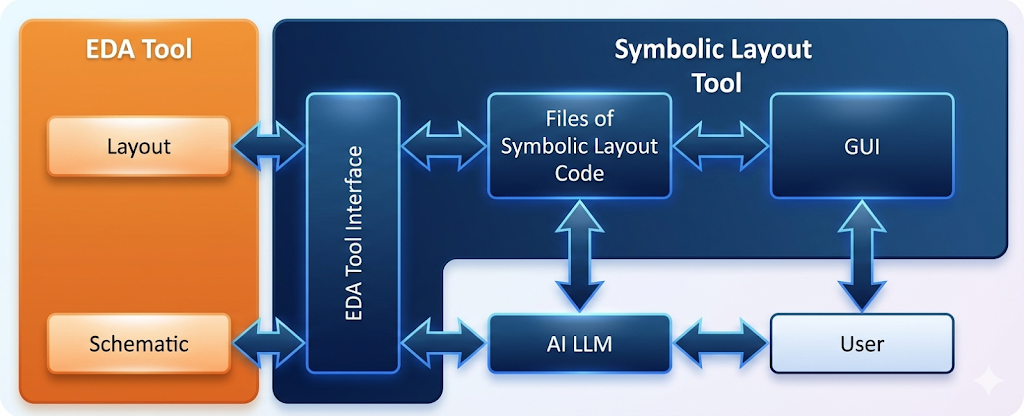
\includegraphics[width=13.5cm]{figures/system_block_diagram.png}}
    \caption{System block diagram showing the four main stages: SPICE Netlist Ingestion, LangGraph AI Placer, Co-Pilot GUI, and Output Compilation.}
    \label{fig:system_block_diagram}
\end{figure}

The system architecture consists of four distinct operational stages:
\begin{enumerate}
    \item \textbf{Stage 1 (EDA Ingestion):} This stage parses standard SPICE netlists, resolves PDK transistor options, and executes subgraph matching to group critical differential pairs and matching networks.
    \item \textbf{Stage 2 (LangGraph AI Placement):} This stage uses a LangGraph multi-agent team to plan device orientations, unroll device fingers, and group transistors. A specialized Critic agent checks Design Rule Checking (DRC) boundaries and coordinates with the Placer to self-heal spacing violations in an iterative loop.
    \item \textbf{Stage 3 (Co-Pilot Interactive Review):} The designer interacts with the layout canvas via a PySide6 user interface. The UI translates natural-language layout instructions (e.g., "align transistors M1 and M2 along the horizontal axis") into formal XML commands that are queued and executed dynamically.
    \item \textbf{Stage 4 (Compaction \& Exporters):} This stage maps the symbolic coordinates to physical sub-micron rules, sharing source/drain diffusions between adjacent transistors. The final compacted geometries are exported directly as binary OASIS files or injected into Cadence Virtuoso using in-memory TCL scripts.
\end{enumerate}

\subsection{Self-Healing Placer-Critic Flow}
\label{subsec:self_healing_flow}

A key feature of the LangGraph-based placement agent is its self-healing feedback loop. When the Placer Agent proposes a floorplan, the Critic Agent evaluates the symbolic spacing against the PDK rules. Figure~\ref{fig:flowchart_self_healing} details this iterative correction process.

\begin{figure}[H]
    \centering
    \fbox{\begin{tikzpicture}[
        node distance=1.6cm and 1.2cm,
        terminal/.style={draw=CodeGreen, fill=CodeGreen!10, text=CodeGreen!60!black, thick, rounded corners=6pt, minimum width=2.6cm, minimum height=0.9cm, align=center, font=\small\sffamily\bfseries, drop shadow={shadow xshift=1.5pt, shadow yshift=-1.5pt, fill=black!15}},
        process/.style={draw=RoyalBlue, fill=LightBlueBg, text=AcademicBlue, thick, rounded corners=4pt, minimum width=3.2cm, minimum height=0.9cm, align=center, font=\small\sffamily\bfseries, drop shadow={shadow xshift=1.5pt, shadow yshift=-1.5pt, fill=black!15}},
        decision/.style={draw=WarmGold, fill=PaleGold!30, text=AcademicBlue, thick, diamond, aspect=2.2, minimum width=3.0cm, minimum height=0.9cm, align=center, font=\small\sffamily\bfseries, drop shadow={shadow xshift=1.5pt, shadow yshift=-1.5pt, fill=black!15}},
        arrow/.style={-Latex, line width=1.3pt, draw=AcademicBlue},
        feedbackarrow/.style={-Latex, line width=1.3pt, draw=WarmGold, dashed}
    ]
        % Nodes
        \node[terminal] (start) {Start Placement};
        \node[process, below=1.0cm of start] (place) {Placer Agent\\Proposes Floorplan};
        \node[process, below=1.0cm of place] (critic) {Critic Agent\\Checks DRC Spacings};
        \node[decision, below=1.0cm of critic] (check) {DRC Clean?};
        \node[process, right=1.5cm of check] (feedback) {Critic Formulates\\Correction Vector};
        \node[terminal, below=1.2cm of check] (end) {Export Placements};

        % Arrows
        \draw[arrow] (start) -- (place);
        \draw[arrow] (place) -- (critic);
        \draw[arrow] (critic) -- (check);
        \draw[arrow] (check) -- node[left, font=\small\sffamily\bfseries\color{AcademicBlue}] {Yes} (end);
        \draw[arrow] (check) -- node[above, font=\small\sffamily\bfseries\color{WarmGold}] {No} (feedback);
        \draw[feedbackarrow] (feedback) |- (place);
    \end{tikzpicture}}
    \caption{Flowchart of the Placer-Critic self-healing loop inside the LangGraph engine.}
    \label{fig:flowchart_self_healing}
\end{figure}

% ==============================================================================
\newpage
\section{Core Contributions}
\label{sec:contributions}

The key contribution of this work is the development of a multi-stage analog placement compilation pipeline that bridges AI reasoning and deterministic hardware construction. This architecture is summarized in the hierarchical system breakdown shown in Figure~\ref{fig:mindmap_system}.

\begin{figure}[H]
    \centering
    \fbox{\begin{tikzpicture}[
        % Style for nodes
        root/.style={
            draw=WarmGold,
            fill=AcademicBlue,
            text=white,
            font=\sffamily\bfseries\small,
            rounded corners=6pt,
            minimum width=5.2cm,
            minimum height=1.1cm,
            align=center,
            drop shadow={shadow xshift=1.8pt, shadow yshift=-1.8pt, fill=black!25}
        },
        % Stage-specific styles
        stage1/.style={draw=RoyalBlue, fill=RoyalBlue!8, text=AcademicBlue, font=\sffamily\bfseries\scriptsize, rounded corners=4pt, minimum width=3.3cm, minimum height=0.8cm, align=center, drop shadow={shadow xshift=1.2pt, shadow yshift=-1.2pt, fill=black!15}},
        stage2/.style={draw=CodeBlue, fill=CodeBlue!8, text=CodeBlue, font=\sffamily\bfseries\scriptsize, rounded corners=4pt, minimum width=3.3cm, minimum height=0.8cm, align=center, drop shadow={shadow xshift=1.2pt, shadow yshift=-1.2pt, fill=black!15}},
        stage3/.style={draw=CopperAccent, fill=CopperAccent!8, text=CopperAccent!80!black, font=\sffamily\bfseries\scriptsize, rounded corners=4pt, minimum width=3.3cm, minimum height=0.8cm, align=center, drop shadow={shadow xshift=1.2pt, shadow yshift=-1.2pt, fill=black!15}},
        stage4/.style={draw=CodeGreen, fill=CodeGreen!8, text=CodeGreen!80!black, font=\sffamily\bfseries\scriptsize, rounded corners=4pt, minimum width=3.3cm, minimum height=0.8cm, align=center, drop shadow={shadow xshift=1.2pt, shadow yshift=-1.2pt, fill=black!15}},
        % Leaf-specific styles
        leaf1/.style={draw=RoyalBlue!50, fill=SoftCream, text=TextCharcoal, font=\sffamily\tiny, rounded corners=3pt, minimum width=3.1cm, minimum height=0.7cm, align=center, drop shadow={shadow xshift=0.8pt, shadow yshift=-0.8pt, fill=black!10}},
        leaf2/.style={draw=CodeBlue!50, fill=SoftCream, text=TextCharcoal, font=\sffamily\tiny, rounded corners=3pt, minimum width=3.1cm, minimum height=0.7cm, align=center, drop shadow={shadow xshift=0.8pt, shadow yshift=-0.8pt, fill=black!10}},
        leaf3/.style={draw=CopperAccent!50, fill=SoftCream, text=TextCharcoal, font=\sffamily\tiny, rounded corners=3pt, minimum width=3.1cm, minimum height=0.7cm, align=center, drop shadow={shadow xshift=0.8pt, shadow yshift=-0.8pt, fill=black!10}},
        leaf4/.style={draw=CodeGreen!50, fill=SoftCream, text=TextCharcoal, font=\sffamily\tiny, rounded corners=3pt, minimum width=3.1cm, minimum height=0.7cm, align=center, drop shadow={shadow xshift=0.8pt, shadow yshift=-0.8pt, fill=black!10}},
        % Connector styles
        conn1/.style={draw=RoyalBlue, line width=1.3pt, -{Latex[length=4pt, width=3.5pt]}},
        conn2/.style={draw=CodeBlue, line width=1.3pt, -{Latex[length=4pt, width=3.5pt]}},
        conn3/.style={draw=CopperAccent, line width=1.3pt, -{Latex[length=4pt, width=3.5pt]}},
        conn4/.style={draw=CodeGreen, line width=1.3pt, -{Latex[length=4pt, width=3.5pt]}},
        rootconn/.style={draw=WarmGold, line width=1.5pt}
    ]
        % Root Node
        \node[root] (root) {Analog Layout Automation Framework};

        % Stage Nodes (Level 1)
        \node[stage1, below=1.2cm of root, xshift=-5.4cm] (s1) {Stage 1\\EDA Ingestion};
        \node[stage2, below=1.2cm of root, xshift=-1.8cm] (s2) {Stage 2\\AI LangGraph Placer};
        \node[stage3, below=1.2cm of root, xshift=1.8cm] (s3) {Stage 3\\Co-Pilot GUI};
        \node[stage4, below=1.2cm of root, xshift=5.4cm] (s4) {Stage 4\\Output Compiler};

        % Leaf Nodes for Stage 1 (Level 2)
        \node[leaf1, below=0.5cm of s1] (l11) {SPICE Parser};
        \node[leaf1, below=0.3cm of l11] (l12) {Subgraph Matching};
        \node[leaf1, below=0.3cm of l12] (l13) {PDK Bounding Box};

        % Leaf Nodes for Stage 2
        \node[leaf2, below=0.5cm of s2] (l21) {Symmetry Strategy};
        \node[leaf2, below=0.3cm of l21] (l22) {Finger Expansion};
        \node[leaf2, below=0.3cm of l22] (l23) {DRC Self-Healing};

        % Leaf Nodes for Stage 3
        \node[leaf3, below=0.5cm of s3] (l31) {Intent Parsing};
        \node[leaf3, below=0.3cm of l31] (l32) {XML Command Queue};
        \node[leaf3, below=0.3cm of l32] (l33) {KLayout Socket};

        % Leaf Nodes for Stage 4
        \node[leaf4, below=0.5cm of s4] (l41) {Diffusion Compactor};
        \node[leaf4, below=0.3cm of l41] (l42) {OASIS Exporter};
        \node[leaf4, below=0.3cm of l42] (l43) {TCL DB Injection};

        % Connectors from Root to Stages
        \draw[rootconn, -{Latex[length=4pt, width=4.5pt]}] (root.south) -- ++(0,-0.4cm) -| (s1.north);
        \draw[rootconn, -{Latex[length=4pt, width=4.5pt]}] (root.south) -- ++(0,-0.4cm) -| (s2.north);
        \draw[rootconn, -{Latex[length=4pt, width=4.5pt]}] (root.south) -- ++(0,-0.4cm) -| (s3.north);
        \draw[rootconn, -{Latex[length=4pt, width=4.5pt]}] (root.south) -- ++(0,-0.4cm) -| (s4.north);

        % Connectors from Stages to Leaves
        \draw[conn1] (s1.south) -- (l11.north);
        \draw[conn1] (l11.south) -- (l12.north);
        \draw[conn1] (l12.south) -- (l13.north);

        \draw[conn2] (s2.south) -- (l21.north);
        \draw[conn2] (l21.south) -- (l22.north);
        \draw[conn2] (l22.south) -- (l23.north);

        \draw[conn3] (s3.south) -- (l31.north);
        \draw[conn3] (l31.south) -- (l32.north);
        \draw[conn3] (l32.south) -- (l33.north);

        \draw[conn4] (s4.south) -- (l41.north);
        \draw[conn4] (l41.south) -- (l42.north);
        \draw[conn4] (l42.south) -- (l43.north);

    \end{tikzpicture}}
    \caption{Hierarchical component breakdown of the multi-stage AI-based analog layout system.}
    \label{fig:mindmap_system}
\end{figure}

The specific contributions detailed in this thesis are:
\begin{itemize}
    \item \textbf{Decoupled Layout Data Model:} A unified intermediate JSON representation that models transistor placement on a virtual symbolic grid, facilitating easy editing and fast rendering.
    \item \textbf{Self-Healing LangGraph Pipeline:} A multi-agent framework featuring a specialized \textit{DRC Critic} that feeds geometric collision vectors back into the LLM placer for automated layout fixing.
    \item \textbf{Double Exporter System:} An export flow supporting direct binary OASIS compilation via \texttt{gdstk} and in-memory cell translation inside OpenAccess tools using a background file watcher and TCL execution.
\end{itemize}

% ==============================================================================
% \section{Thesis Organization}
\label{sec:organization}

The remainder of this mixed-signal layout compilation thesis is organized as follows:
\begin{itemize}
    \item \textbf{Chapter~\ref{ch:lit_review} (Literature Review):} Discusses classical layout placement algorithms (including simulated annealing and sequence pairs), neural networks for layout prediction, and LLM implementations for design automation.
    \item \textbf{Chapter~\ref{ch:system_arch} (System Architecture):} Presents the unified decoupled architecture, details the central layout data model, and explains how physical coordinates are abstracted into virtual symbolic slots.
    \item \textbf{Chapter 4 (EDA Input Parser):} Explains the input ingestion stage, detailing SPICE netlist parsing, transistor parameter resolving, and the subgraph isomorphism implementation used for matched pair clustering.
    \item \textbf{Chapter 5 (LangGraph Placer):} Details the multi-agent cooperative graph, the role of each agent (placer, router, and critic), and the self-healing layout loop.
    \item \textbf{Chapter 6 (Co-Pilot GUI):} Describes the PySide6 user interface, the socket server stream connecting the GUI to the agent backend, and the XML command execution schema.
    \item \textbf{Chapter 7 (Compaction \& Exporters):} Outlines the physics-based 1D diffusion-sharing compaction compiler, the direct binary OASIS layout compilation, and the Cadence Virtuoso TCL database injection watcher.
    \item \textbf{Chapter 8 (Results \& Verification):} Presents experimental evaluation results across typical analog blocks (bias mirrors, differential amplifiers, comparators), analyzing layout compaction ratios and agent convergence times.
    \item \textbf{Chapter 9 (Conclusion \& Future Work):} Summarizes the primary contributions of this thesis and identifies directions for mixed-signal routing automation and AI placement.
\end{itemize}
